\section{Introduction}

\subsection{Purpose of the System}

\subsection{Scope}

\subsection{System Overview}

\subsubsection{System Perspective}

afetbilgi.com is not a part of a larger system. It is a standalone website website to verify important information in the fight against the 6 February 2023 Pazarcik Earthquake and to deliver it to both disaster victims and those who want to help.

System uses human-made database verified and updated by data collectors and validators. The data is classified into two, called hot and cold. After the verification and classification steps, system parses the data and translate it to JSON file.

If it is necessary, admin/maintainers make changes to display the newly created data and upload it to the system.

\begin{figure}[H]
  \centering
  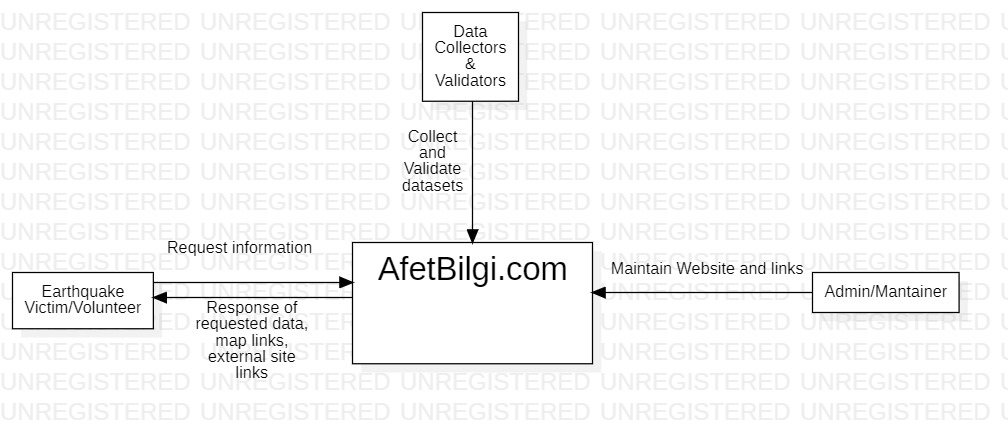
\includegraphics[width=\textwidth]{img/context-diagram.jpg}
  \caption{Context Diagram for \href{https://afetbilgi.com}{afetbilgi.com}}
\end{figure}

\subsubsection{System Functions}

\subsubsection{Stakeholder Characteristics}

\subsubsection{Limitations}

\subsection{Definitions}
